% !TeX encoding = UTF-8
% !TeX program = xelatex
% !TeX spellcheck = en_US

\documentclass{kqdlxxb}
\usepackage{booktabs}
\usepackage{algorithm}
\usepackage{algorithmic}
\usepackage{siunitx}
\usepackage{silence}
\usepackage{booktabs}
\usepackage{amsmath}
\usepackage{multirow}
\usepackage{diagbox}
\usepackage{blindtext}
\usepackage{pdfpages}
\usepackage{subfig}
\usepackage{threeparttable}
\usepackage{enumitem}
\usepackage{bicaption}%属于caption的扩展包，有中英文双语
\usepackage{multicol}
% hyperref 总是在导言区的最后加载
\usepackage{hyperref}
\usepackage[nameinlink]{cleveref}  % after hyperref package

\addbibresource{example.bib} % 设置参考文献文件位置

\captionsetup[figure][bi-second]{name=Fig.}%设置英文图开头为Fig.
\captionsetup[table][bi-second]{name=Table}%设置英文图开头为Table

\setenumerate[1]{itemsep=0pt,partopsep=0pt,parsep=\parskip,topsep=0pt}
\setitemize[1]{itemsep=0pt,partopsep=0pt,parsep=\parskip,topsep=0pt}
\hbadness=10000 \vbadness=10000 
\WarningFilter{Fancyhdr}{\headheight is too small}

% 图片路径
\graphicspath{{fig/}}


\classsetup{
  % 配置里面不要出现空行 
  title        = {排版格式与论文书写要求（20字以内）},
  title*       = {Review suggestion to technical paper(第一个单词首字母大写，专有名词大写，减少不必要的冠词、以及“研究”之类的说明性单词)},
  authors      = {
    author1 = { 
      name         = {张三 \textsuperscript{1} },
      name*        = {ZHANG San\textsuperscript{1}},
      affiliations = {aff1}
    },
    author2 = {
      name         = {李四  \textsuperscript{1\text{，}2}},
      name*        = {LI Si \textsuperscript{1,2}},
      affiliations = {aff1, aff2}
    },
    author3 = {
      name         = {王五六 \textsuperscript{1\text{，}2\text{，}*}},
      name*        = {WANG Wuliu\textsuperscript{1,2,*}},
      affiliations = {aff1, aff2},
      % 通讯作者
      corresponding = true,
    },
  },
  % 论文定稿后，作者署名、单位无特殊情况不能变更。若变更，须提交签章申请，
  % 国家名为中国可以不写，省会城市不写省的名称，其他国家必须写国家名。
  affiliations = {
    aff1 = {
      name  = {（1.清华大学 航天航空学院，北京 100084；},
      name* = {(1.\textit{ School of Aerospace Engineering, Tsinghua University，Beijing 100084，China};},
    },
    aff2 = {
      name  = {2.中国空气动力研究与发展中心，绵阳 621000)},
      name* = {2.\textit{China Aerodynamics Research and Development Center，Mianyang 621000，China})},
    }
  },
  abstract     = {
    为了更好地提高文章写作质量和规范写作格式，现给出《空气动力学学报》的论文模板供参考。摘要是一篇论文的浓缩与精华，逻辑顺序包括四个要素：目的、方法、结果、结论，同时要将论文的创新点反映到摘要之中。根据国家规范，采用第三人称概括全文，一般不出现“本文”字样。第一句话体现研究目的，不要大量介绍背景知识，把引言内容当摘要；研究方法与正文保持一致；结果是反映本文的主要研究成果，建议包含尽可能定量或定性的信息，忌笼统、不具体、发散；结论如实反映论文的新观点、新内容、具体的对策建议等，不需要加自我评论和补充解释。总之，通过摘要的阅读，读者对该文的基本观点、重要内容及结论能够有一个清晰的认识。350字左右。写作时注意保存高清图片（tif格式，最好是矢量图），以便在录用排版时单独提供。
  },
  abstract*    = {A form of short paper is presented to show the review suggestion. ……The technical papers can be revised by authors according to the suggestion，and it can also be processed in the form of this short paper.To accurately solve the curved slip wall using finite difference methods, this work proposes a boundary constraint algorithm assigning ghost nodes based on the discrete equivalent equation that eliminates the coordinate transformation-induced errors. Except for the wall-normal velocity, this method further constrains the wall-normal momentum flux at the wall to zero. （学报被Scopus等国外重要检索系统收录，国外同行可以从摘要数据库获得本刊的英文摘要，因此，英文摘要的写作要求比中文摘要更详细具体，包含且不限于中文摘要的所有内容，成为一篇完整独立的长摘要，并请注意主语、时态和单复数等问题，长度建议实词数250～350，长短保证在A4纸大半页的样子。） },
  % 中文关键字与英文关键字对应且一致，应有5-7个关键词，不要用英文缩写
  keywords     = {论文；排版；格式；规范；要求（提供5个左右反映论文主题的关键词，按重要性排列）},
  keywords*    = {technical paper; dissertation; typesetting; format; specification; requirements（与中文关键词相对应）},
}



\newcommand\dif{\mathop{}\!\mathrm{d}}


%中英文参考文献对照
\defdoublelangentry{刘炜201348}{Liuwei201348}
\defdoublelangentry{李志辉1996阿波罗指令舱稀薄气体动力学特征的蒙特卡罗数值模拟}{LiZhihui1996}
\defdoublelangentry{庄逢甘2006未来空间飞行器的某些发展和空气动力学的任务}{zhuangfenggan2006}
\defdoublelangentry{2022-xx}{2022-xxen}

\begin{document}


\maketitle

%脚注
\begin{multicols}{2}
  \footnote{\textbf{收稿日期：}202x-xx-xx ；\textbf{修改日期：}202x-xx-xx；\textbf{录用日期：}2023-xx-xx；\textbf{网络出版时间：}2023-xx-xx\\     %
  \textbf{基金项目：}省级以上基金项目（基金编号）\\
  \textbf{作者简介：}张三（出生年-），性别，籍贯，职称，研究方向：高超声速空气空气动力学. E-mail：zhangsan@163.com  \\
  \textbf{通信作者：}王五六\textsuperscript{*}（是该文的修改、发表联系人，承担有关该论文的全部责任，享有该文的知识产权，可由作者商议决定，国际惯例为导师。）职称，研究方向：空气动力学. E-mail: wangwl@163.com}
\end{multicols}
\clearpage


\section{引 \ \ 言}

根据科技论文发展的要求\cite{刘炜201348,李志辉1996阿波罗指令舱稀薄气体动力学特征的蒙特卡罗数值模拟}，为了使文章内容完整、翔实和具有更多的可读性\cite{庄逢甘2006未来空间飞行器的某些发展和空气动力学的任务}，本期刊不再对文章篇幅进行过多的限制，作者可根据内容的需求适当增加篇幅。同时，请作者重视摘要、引言和结论的写法以及参考文献的引用，请关注红色和蓝色字体，我们将在该篇每个部分重点强调科技论文的写作要求。

科技论文的引言必须交代研究工作的背景，概括性地论述所研究问题的现状。对研究现状的论述，不宜过大过泛，要与本文的研究方向紧密相关\cite{2022-xx}。同时，引言中对参考文献的引用，不仅是考查作者对资料的占有程度和熟悉程度，更重要的是从资料的全面程度和新旧程度可以判断研究工作的意义和价值，以及研究结果的可信度。因此在这里建议作者尽量引用比较新的参考文献（科技论文参考文献的数量平均在15篇左右）。

其次说明本研究与前工作的关系，目前的研究热点、存在的问题及本文工作的意义，明确点明本文的创新点、与前人研究的不同之处或解决了什么问题，使读者一目了然。

引言最后一段可点明本文的理论依据、实验基础和研究方法，简要阐述下面即将开展的研究内容，预示研究的结果、意义和前景，但不必展开讨论。

\section{稿件规范要求}

\subsection{论文结构}
论文层次体例为：中文文题、作者姓名、单位、中文摘要、关键词、中图分类号、英文文题、英文摘要(包括作者姓名及单位英译、关键词)、收稿日期(首页下注)、基金项目(首页尾注)、作者简介(首页尾注)、正文(按1 2 3 ，1.1  1.2  1.3，1.1.1  1.1.2  1.2.1， 1)  2)  3)、参考文献（中英文双语）。
\begin{figure}[!htb]
  \centering
  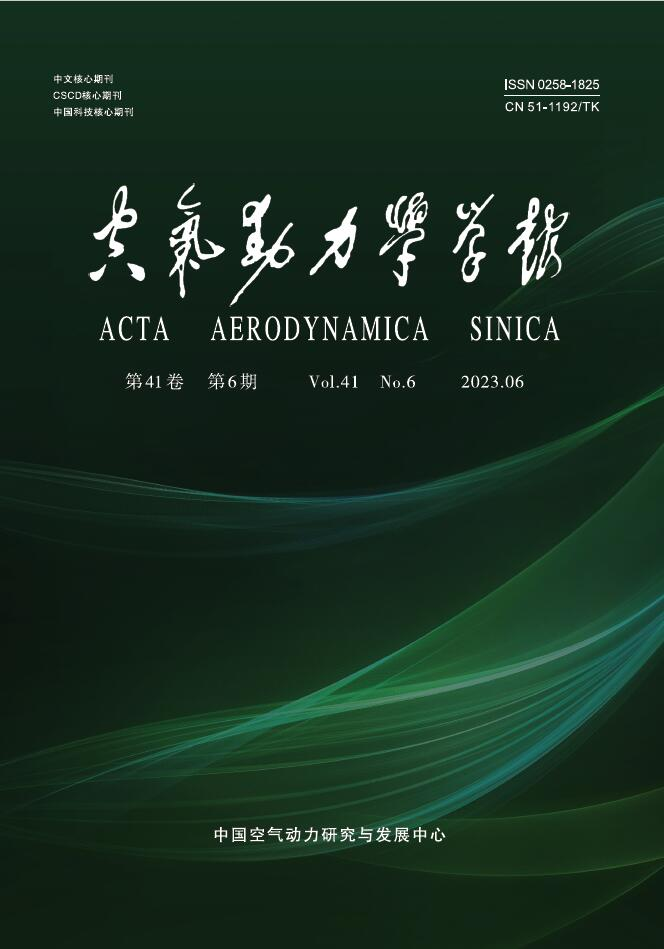
\includegraphics[height=5cm]{cover-kqdlxxb.jpg}
  \renewcommand{\figurename}{图}
  \caption{学报封面}
  %英文标题begin
  \addtocounter{figure}{-1}
  \vspace{-4pt}
  %\SetEnglishCaption
  \renewcommand{\figurename}{Fig.}
  \caption{the cover of kqdlxxb}
  %英文标题end
  \label{fig:cover}
\end{figure}

请在投稿系统中清楚填写作者的联系地址、邮编、电话、手机号及E-mail。联系方式如有变更，请及时通知编辑部或自行登录系统修改\cite{闫吉庆2022基于}。
\subsection{图、表}
文中图表必须清晰，图题、表题均需中英文对照，分图题只需要中文；图、表中的文字用英文表示，太长或不宜用英文的，可以用中文。合理使用SI词头或10的幂，使数值范围在0.1～999之间。图与表应放在相应正文之后，分别按出现顺序用图1、图2或表1、表2统一编号，如图\ref{fig:jiyi}所示。

\begin{figure}[!htb]
  \centering
  \subfloat[机翼1]{
      \centering
      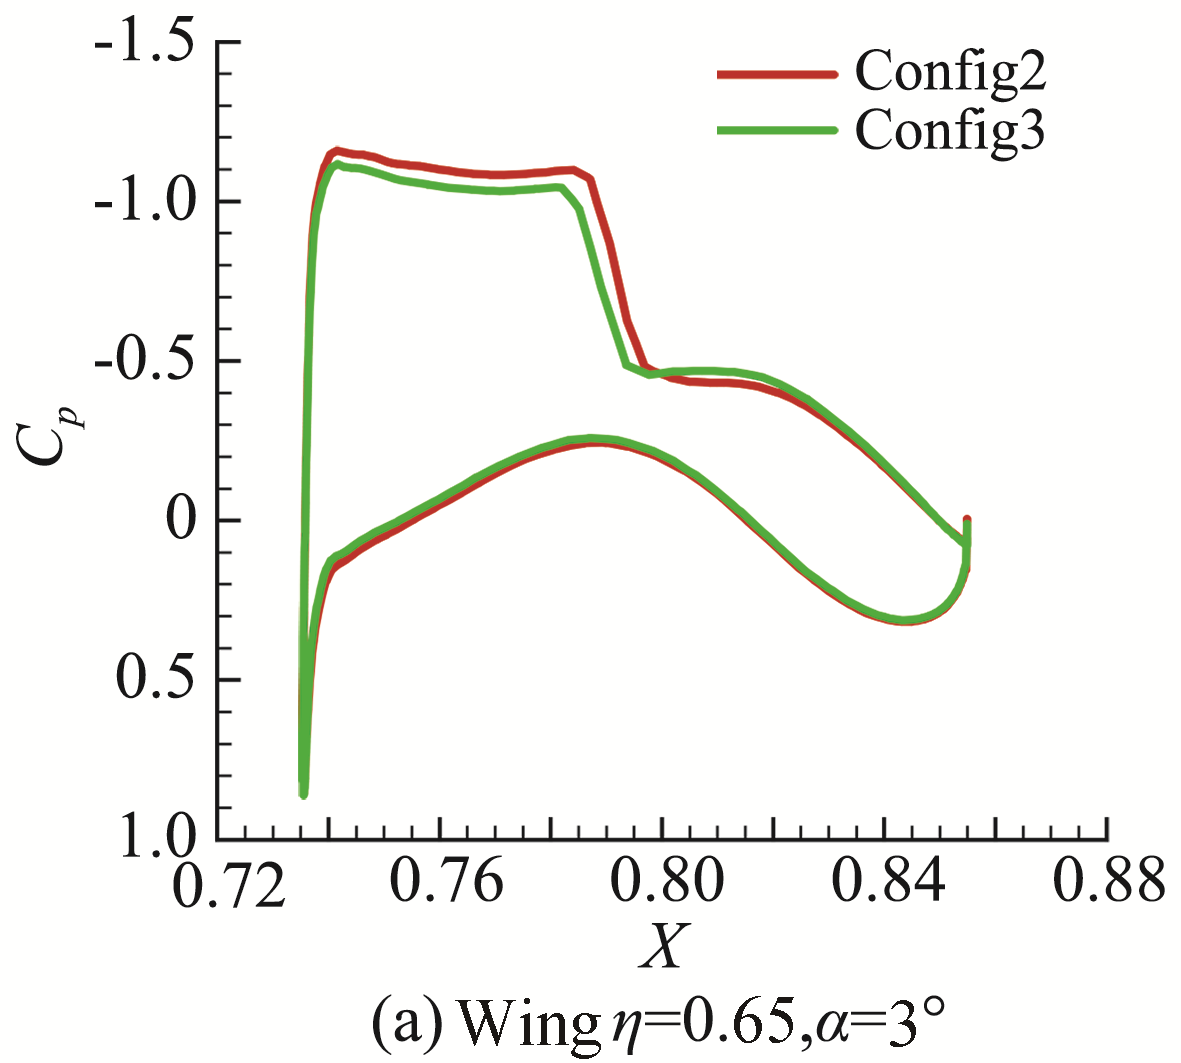
\includegraphics[height=5cm]{jiyi-1.png}
  }
  \quad
  \subfloat[机翼2]{
      \centering
      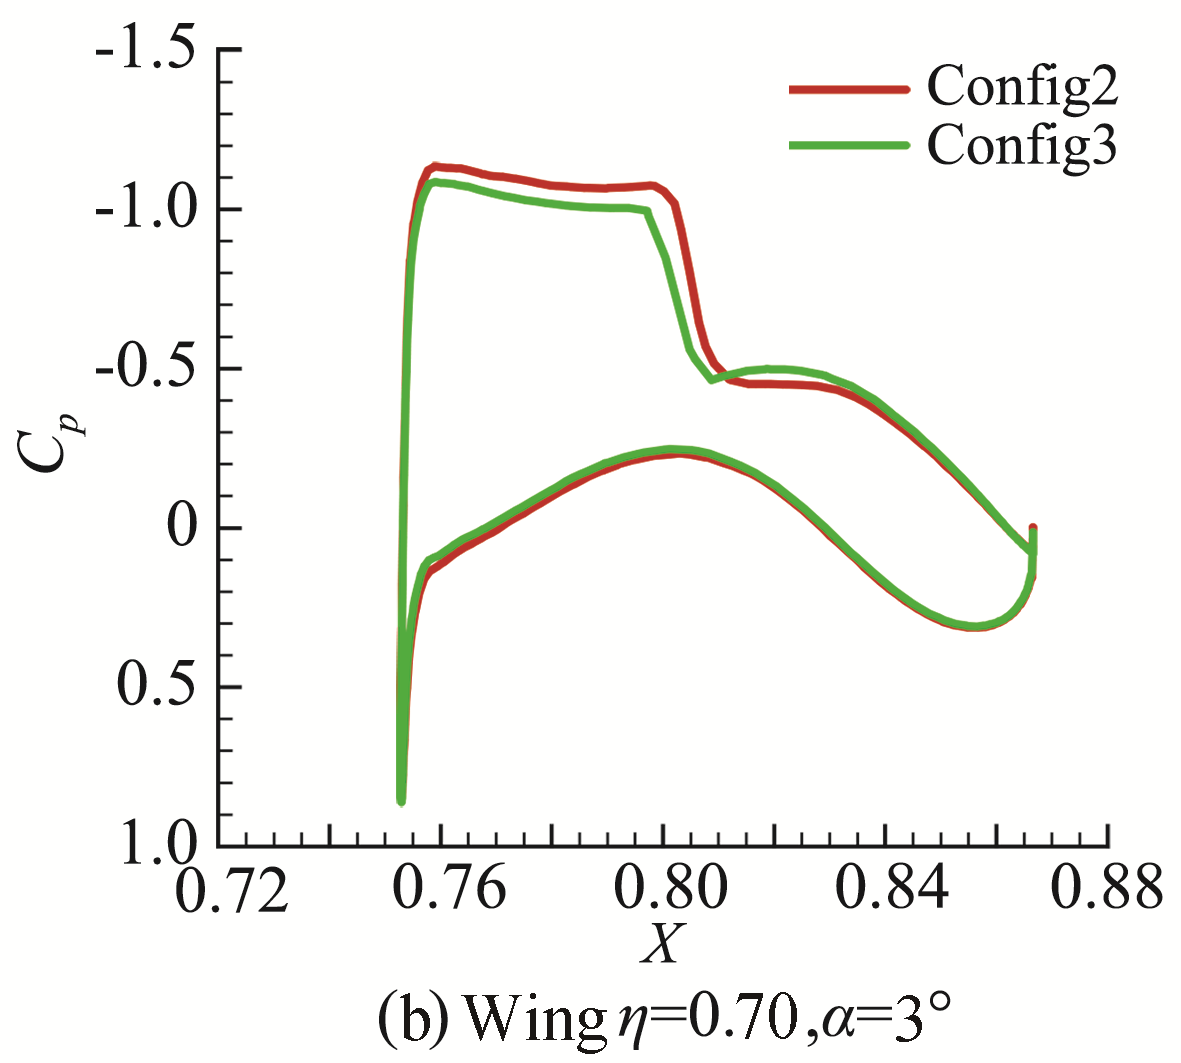
\includegraphics[height=5cm]{jiyi-2.png}
  }
  \renewcommand{\figurename}{图}
  \caption{示例图片\protect \cite{闫吉庆2022基于}}
  %英文标题begin
  \addtocounter{figure}{-1}
  \vspace{-4pt}
  %\SetEnglishCaption
  \renewcommand{\figurename}{Fig.}
  \caption{Example 1 \protect \cite{闫吉庆2022基于}}
  %英文标题end
  % \bicaption{示例图片}{Example 1}
  \label{fig:jiyi}
\end{figure}



图的序号、标题及注释居中放在图的下方。表示数量的图、表中的量和图的数轴应给出单位，并采用国际标准单位。一般情况下，编辑部排版人员会修正图片，作者仅提供清晰原图即可。我刊已采用彩色印刷，请大家尽量提供彩色图，辨识度更好。表格采用三线表。表的序号及标题置于表格上方，表注放在表格的下方，如表\ref{tab:case-1}所示。
\begin{table}[htb]
    \centering
    \renewcommand{\tablename}{表}
    \caption{示例表格}
    %英文标题begin
    \addtocounter{table}{-1}
    \vspace{-4pt}
    %\SetEnglishCaption
    \caption{Example 1}
    %英文标题end
      % \bicaption{示例表格}{Example 1}
      \label{tab:case-1}
      \begin{threeparttable}
      \begin{tabular}{cccc}
          \toprule
          $I$/mA& $v$/m $\cdot$ s$^{-1}$& $h$/m& $p$/MPa \\
          \midrule
          30& 2.5& 4& 110 \\
          34& 3.0& 5& 111 \\
          \bottomrule
      \end{tabular}
      \begin{tablenotes}[para,flushleft]
        \footnotesize
        \item 注：表注用六号宋体，左对齐。  %此处加入注释*信息
      \end{tablenotes}
    \end{threeparttable}
\end{table}


\subsection{物理量、公式等}

名词、术语、数字、计量单位、标点符号和数学符号等，必须符合国家标准。

变量、函数用斜体；英文单词的首字母组合代表的变量或上下标为正体，如RMS、sin、$F_{\rm N}$等，但是上下标是变量的则为斜体，如$C_p$、$C_L$；矢量、张量、矩阵符号用黑斜体；单位矩阵、转置符号“T”，对角符号“dig”，单位符号（如m、N等）、表示图号和公式编号的字母用正体。示例请见公式\eqref{eq:case-1}、\eqref{eq:case-2}所示。

量的表达书写一定要前后文保持一致，如前文用$d$=0.01m，后文就不要用$d$=10mm，等等。

参数范围用浪纹线“~”表示；年月日之间、连接词、文献号等用连接符“-”表示；页码范围等用起止符“-”表示；外文地名和术语请尽量译成中文，除常见者外在首次出现时在括号内注明原文。

文中、公式中的变量要在第一次提及时说明(常见的除外)，并自成系统，不相互矛盾。公式及物理量符号等易混淆之处，作者应加以特别说明。

公式编号通篇用（1）（2）……，不要再在小节内编号如（1.1）（1.2）……等。

例如，由……可得

\begin{equation} \label{eq:case-1}
  \theta={\rm tan}^{-1} \frac{F_{\rm N}}{F_{\rm A}}
\end{equation}
式中： $F_{\rm N}$为法向力； $F_{\rm A}$为轴向力； $\theta$为法向力与轴向力的夹角。

\subsection{参考文献}
为了减少作者在参考文献格式上花费的时间，本刊在稿件录用后将会用专业文献校对软件对参考文献进行校核以及格式修正。作者只需要注意在正文引用处右上角按顺序注明参考文献序号\parencite{刘炜201348,李志辉1996阿波罗指令舱稀薄气体动力学特征的蒙特卡罗数值模拟,庄逢甘2006未来空间飞行器的某些发展和空气动力学的任务}。提供的参考文献必须为已经出版或有doi号可查或有网址的公开发表资料，尽可能按文献类型给出所有的信息。为方便国外数据库的收录，我刊要求中文文献给出英文对照，英文部分人名著录规则一律为：姓前、名后，姓大写，名缩写，并省略缩写点。

参考文献采用六号字放于文章结论后附录（如果有的话）前，著录格式举例见最后的参考文献。

文献类型标志：普通图书M，会议录C，汇编G，报纸N，期刊J，学位论文D，报告R，标准S，专利P，数据库DB，计算程序CP，电子公告EB。

\section{出版流程}

我刊出版流程为：投稿——编辑初审（查重、保密审查等）——编委初审——外审——退修——编委主审——终审——英文编审——排版前退修——排版——看校样——网络首发——纸质出版。

请作者在投稿之前先看一下我刊网页的“投稿指南”。里面包括了投稿需要上传的文件（版权协议和保密审查单）。如果投稿时，未按照我刊论文排版格式，未提交保密审查单和版权协议的，将会驳回重投。如有特殊原因，可以投稿时留言说明。

外审采用双盲审稿，时间为三个月，主要取决于外审专家的审回快慢，期间编辑会根据情况进行催审、换审等操作，作者也可通过手机我刊微信公众号关注审稿状态。
\begin{equation} \label{eq:case-2}
  f(x)=a+b
\end{equation}

录用后的稿件，原则上不允许再进行较大的改动，如需对作者、单位等进行调整，必须有书面的说明，并取得全体作者签字同意。如果是内容上有较大的变动，需重新进行专家审查。

为缩短学术论文发表周期，提高学术成果的传播和利用价值，更快地将作者的研究成果发布出来，《空气动力学学报》于2013年12月加入了“中国知网”学术期刊优先数字出版平台(http://www.cnki.net)，将对已录用的论文先于印刷版在“中国知网”网络首发，在法律上等同正式出版。优先出版的文章是经同行专家评审、主编终审后拟为本刊录用的稿件。由于优先数字出版未经严格校对，不免存在一些问题和不严谨的地方，稿件一旦纸质出版，将会及时替换掉优先出版的版本。如果您的文章不愿电子优先出版，请您及时和我们联系。

同时，我刊向中国科学技术信息研究所中文DOI机构申请注册了DOI编码，并为发表在我刊的每篇文章分配了doi号，读者可以通过DOI代理服务器（http://dx.doi.org/）或中文DOI代理服务器（http://dx.chinadoi.cn/）有效访问，即可输入地址“http://dx.doi.org/文章doi号”进行解析访问该文章。

\section{结论}
结论不应是正文中各段小结的简单重复，它应以正文中的实验或考察得到的现象、数据的阐述分析为依据，完整、准确、简洁地指出以下内容，并注意突出创新之处，呼应引言提出所要解决的问题。

\begin{enumerate}[label=\arabic*{)}]
    \item 由对研究对象进行考察或实验得到的结果所揭示的原理及其普遍性； 
    \item  研究中有无发现例外或本论文尚难以解释和解决的问题；
    \item  与先前已发表过的（包括他人和作者自己）研究工作的异同；
    \item  本论文在理论上和实用上的意义及价值；
    \item  进一步深入研究本课题的建议。
\end{enumerate}

作者高质量的论文编排，会提高编辑部的工作效率，减少出错率，保证文章按时、正确地出版。



% \begin{acknowledgments}
%   致谢内容。
% \end{acknowledgments}



% 显示参考文献列表，并加参考文献加入目录
\printbibliography[heading=bibintoc]


\end{document}
